\chapter{Theoretical Background}\label{ch:theory}

\section{State-Of-The-Art}\label{sec:state_art}

%\subsection{Sampled sounds vs Procedural audio}



%\subsection{Sound synthesis in virtual and interactive applications}

Researchers have been working on automatically generated synthesized sounds based on physical interactions for quite some time now. Different publications that have contributed to the creation of procedural sounds in 3D virtual environments and that have inspired this thesis are discussed in this section.

Sound spatialization is a crucial component for building 3D virtual scenes and the listener's immersion. Different techniques such as Ambisonics, VBAP and Wave Field Synthesis have been developed to simulate 3D sounds on loudspeakers. Binaural techniques use HRTF functions to simulate the position of a sound source with respect to the listener through the use of headphones. In this thesis spatialization and sound synthesis are considered two separate processes. Here all sounding objects are considered point sources that are spatialized with Unity's Audio Spatializer SDK \cite{bib:unity_doc} which produces the desired effect. This is why sound propagation is not studied in depth. 

Regarding studies related to sound simulation frameworks, in \cite{gaver1993we, gaver1993world} Gaver proposes the analysis and synthesis of contact sounds based on what he calls ``everyday listening'' which consists in focusing on the perceptual features of a sound event. Another pioneering work \cite{takala1992sound} presents a methodology to produce synchronized sounds with animations. \cite{van1998sounds} decribes a framework that uses modal analysis to generate sounds based on the object's material, shape and impact location. This analytical model however can not handle objects with arbitrary or more complex shapes. A \gls{FEM} in \cite{director2001synthesizing} takes advantage of existing simulation techniques models the surface vibration of virtual objects. Despite being more accurate, this method is expensive and non-interactive. In his book \cite{Cook:2002:RSS:515316}, Cook covers extensively physically based sound synthesis concepts and defines a parametric model as one that can be manipulated to change the interaction, object and sound.  

Different techniques have been used to extract modal parameters necessary for modal synthesis. \cite{pai2001scanning} scans the response of real objects to model the interaction behaviour of 3D objects. Despite offering the possibility to synthesize sounds for arbitrary shaped objects, the hardware needed is a clear limitation. A \gls{FEM} approach is used in \cite{o2002synthesizing} for modal analysis and \cite{raghuvanshi2006interactive} uses spring-mass systems to model each object's deformation and vibration.\cite{van2001foleyautomatic} and \cite{lloyd2011sound} make use of modal models derived from recordings of struck objects which is similar to the approach described in this thesis. This model is used to create impact, rolling and sliding sounds.

As far as scratching sounds are concerned, \cite{van2001foleyautomatic} generates a fractal-noise based force profile that is sampled at audio rates to simulate friction force variations. A similar approach is used for rolling sounds by adding a low-pass filter to obtain a rolling quality. \cite{rath2003expressive} develops a model in which the uneven ground surface is significant compared to the size of the rolling object. In \cite{farnell2010designing} the author presents a rolling model that takes into account the uneven ground texture plus the object's surface irregularities. This thesis is heavily inspired by the fore-mentioned paper while improving the model's interactivity in a game engine.

Previous researches on material identification focus on the decay time of vibrating objects. \cite{wildes1988recovering} proposed material type recognition depending on a parameter named ``the coefficient of internal friction'' which depends on the damping of the material. The authors in \cite{giordano2006material} point out that damping remains a robust acoustic descriptor to identify material macro-categories independently of the size of objects. \cite{aramaki2011controlling} proposes a control strategy for the perceived material in an impact sound synthesizer but does not include these controls within a game engine.

Offering the possibility to control the synthesizer that produces the contact sounds of 3D objects is one of the objectives dealt in this work. Little has been made to enable game developers and sound designers to control physic-based sounds through high level parameters within the game engine. In \cite{lloyd2011sound} a set of plugins for Wwise \cite{bib:wwise} have been implemented that enable the audio designer to choose how varied the sounds will be. In the very recent paper \cite{pruvost2015perception} from the PHYSIS project \cite{bib:physis}, the authors introduce a  controllable framework for interactive and real-time synthesized sounds of solids driven by a game engine. This approach shares similarities with the presented tool in this paper.

\section{Sampled sounds vs Procedural audio}

Sampled sound is still the most typical technique for digital audio in the game industry since its sophistication in the late 1990s when game music moved to recorded tracks on CD. Present game audio systems can compare to professional samplers on account of the improvement of hardware decompression and compressed audio formats \cite{farnell2007introduction}. But this method has limitations due to its static and repetitive nature which does not allow to model the sound of an object based on its physical interactions in a game scene. This leads to inconsistencies between the visuals and their associated soundtrack \cite{picard2009expressive}. Despite the use of different processes such as filtering, pitch-shifting and time-scaling to name but three, sampled sounds can not compare to the versatility that procedural audio offers. With the increasing interest that the game industry has put into \gls{VR} and \gls{AR}, it is becoming essential to provide realistic and compelling sounds in these virtual environments to provide immersion and presence to the user. An obvious advantage of procedural audio over recordings is the large memory storage space that is necessary for the latter, due to the huge amount of audio assets present in modern games. The ability of procedural audio to generate sounds automatically based on the interactions of the objects in a scene eases the asset management task for the audio team. Instead, the sound designer becomes more of a programmer by taking into account the object’s behaviour and physical properties to create sounds. This does not mean that the sound designer is replaced by procedural content as certain tasks need special attention to deliver high quality sounds. Regardless of its advantages, procedural audio still lacks of development tool chains and presents conflicts with current methods due to its still scarce use in the industry \cite{farnell2010designing}.

\section{Sound Production}

For computer sounds to be produced, force models are used as input to the sound synthesis algorithm. In other words, physics is used as the excitation parameter to produce sound. \cite{van2003modal} refers to four different interaction models that produce the excitation force.

\begin{enumerate}
\item Impact force, produced during collisions,
\item Continuous contact force, produced during rolling or scratching of an object,
\item Combustion engine forces and
\item Live data streams
\end{enumerate}

This thesis examines sounds produced by the first two models. Impact forces are applied when two objects collide. They last for a short period of time and depend on the physical attributes of the objects. Constant contact forces are produced while an object is rolling on a surface of scratching/sliding on it. They can be modeled as successive impact forces, where one adds on top of the other. The distinction between roll or scratch depends on the shape of the object and on the hardness of both surfaces.

In this thesis we focus on sound produced by rigid-body objects. When two of these objects collide, the energy from the impact deforms them. This deformation is propagated through the whole object, making its outer surfaces vibrate and emit sound waves to the environment. Sound waves impact on other objects in the environment and get reflected and absorbed from them before reaching the ear \cite{van1998sounds}. All the interactions that happen before reaching the ear, contribute to the characterization of the sound, making the listener able to visualize the impact just by sound. Since in this thesis we examine only object-related interactions and not sound propagation, below we explain in depth how each of the object's physical attributes affect sound.


\subsection{Acoustic effects of sound attributes}\label{sec:attributes}

\paragraph{Interaction\\}
An object that receives an impact is deformed during a very short period of time. The vibration lasts until the initial energy is fully damped. Hence, the amplitude of the oscillation depends only on the object's damping. On the other hand, scraping sounds are characterized by a continuous supply of energy that varies throughout the object interaction. The force of the interaction plays the most significant role for the amplitude of the oscillation. The stronger the force, the bigger it imposes the amplitude value to be - and the louder the sound. Additionally, the force affects the spectrum of the resulting sound. The greater the force, the more high frequency components \cite{gaver1993world}.

\paragraph{Material\\}
The material of interacting objects affects their vibration amplitude over time. Several studies \cite{wildes1988recovering, giordano2006material} have examined that damping is a material-specific attribute that is independent from the shape of the object. The more the system is damped, the faster it loses energy and thus the oscillation lasts less. For example, wood has way bigger damping ratio than metal and this is why they produce a ``thud'' and a ``ringy'' sound respectively. Moreover, in \cite{klatzky2000perception} they have proven that material and spectral characteristics are correlated, for example glass is found to include in general higher frequencies than rubber. 

\paragraph{Configuration\\}
Moreover, the configuration of the object also affects its vibration. The size of it determines how high or low pitched the sound produced will be. That is to say, the smaller the object, the higher pitched is the sound. Elasticity, on the other hand, influences the impact force since the more elastic an object is, the bigger the excitation area gets when colliding.  

Table \ref{tab:acoustic_effects} shows the effects on the sound wave generated by each physical attribute. 

\begin{table}[H]
	\centering
    \begin{tabular}{  l  l }
    \toprule
     \addlinespace
    \textbf{\textit{Attribute}} & \textbf{\textit{Changes on Sound Wave}} \\ \toprule
    \addlinespace
\cmidrule(l{0.8cm}r{4.7cm}){1-2}
    \multicolumn{2}{l}{\hspace{0.8cm}\textit{Interaction}} \\ \cmidrule(l{0.8cm}r{4.7cm}){1-2}
     Type & Amplitude, spectrum \\ 
     Force & Amplitude, bandwidth \\
     \addlinespace
\cmidrule(l{0.8cm}r{4.7cm}){1-2}
    \multicolumn{2}{l}{\hspace{1cm}\textit{Material}} \\ \cmidrule(l{0.8cm}r{4.7cm}){1-2}
    Density & Frequency \\
    Damping & Amplitude, frequency \\
    Homogeneity & Amplitude, frequency \\
     \addlinespace
\cmidrule(l{0.8cm}r{4.7cm}){1-2}
    \multicolumn{2}{l}{\hspace{0.6cm}\textit{Configuration}} \\ \cmidrule(l{0.8cm}r{4.7cm}){1-2}
    Shape & Frequency, spectral pattern \\ 
    Size & Frequency, bandwidth \\
    Elasticity & Amplitude, frequency \\
    \bottomrule
    \end{tabular}
    \caption{Acoustic effects of source attributes \cite{gaver1993world}.}
    \label{tab:acoustic_effects}
\end{table} 

\section{Modal parameters extraction}\label{sec:modal_extraction}
%change modal analysis stuff, say that the extracted parameters are the same for every one of the 3 methods
Before the sound synthesis can be done, we need to extract certain modal parameters that are characteristic of the vibrating solid object and will be fed as input. The data needed for a physically motivated synthesis, namely modal synthesis, is shown in the table \ref{tab:extracted_data}.

\begin{table}[H]
	\centering
    \begin{tabular}{ c l l }
    \toprule
    \textbf{Symbol} & \textbf{Description} & \textbf{Derivation} \\ \toprule
    $A_n$ & Initial amplitude & Modal data extraction \\ 
    $d_n$ & Decay rate & Material properties \\ 
    $f_n$ & Modal frequency & Modal data extraction \\
    \bottomrule
    \end{tabular}
    \caption{Derivation of data used in modal synthesis.}
    \label{tab:extracted_data}
\end{table} 

Since every different point struck on the object produces different deformations and thus sound, matrices are used to represent the data needed for each point. More specifically, we need a vector $\textbf{f}\sim (K \times 1)$  corresponding to the modal frequencies of every point, a vector $\textbf{d}\sim (K \times 1)$ corresponding to the decay ratios and a matrix $\textbf{A}\sim (K \times N)$, which corresponds to the amplitudes of each mode in every point of the object, where $K$ is the number of modal frequencies calculated in one point and $N$ the number of points. All the above gives the modal model which can be represented as $\textbf{M} = \{\textbf{f}, \textbf{d}, \textbf{A}\}$ \cite{van2001foleyautomatic}. To obtain this model, different techniques such as the \gls{FEM}, spring-mass systems and the example-guided approach have been used for data extraction and are reviewed here below.

%In this thesis we focus on the sound produced by solid objects due to different interactions such as falling on the floor or colliding with another object. The sounds produced can be impact, rolling or scratching sounds. When an object is excited, the forces applied cause deformations to it, emitting sound waves through the vibration of its outer surfaces \cite{van2001foleyautomatic}.%

\subsection{FEM}\label{sec:fem}

\gls{FEM} is a simulation technique that is commonly used for modal analysis, which studies the response of a structure when it vibrates freely. \cite{o2002synthesizing} uses this approach on meshes to precompute the shape and frequencies of an object's deformation modes. It is an accurate method to create \textit{sound maps} of complex-shaped objects without the need of recording equipment or the actual physical object. Most importantly it computes the resonant modes at different locations on the object. A downside of this method is that it complicates the audio pipeline in a game production as the sound designer would need to deal with complex computations and material properties that are not intuitive for him to obtain the desired modal parameters.

\subsection{Spring-mass systems}\label{sec:springmass}

A spring-mass system consists in constructing a model that approximates the object's surface based on its geometry and material properties. In \cite{raghuvanshi2006interactive}, the authors convert each mesh's vertices into masses and its edges into damped springs. They solve an ordinary equation based on the input mesh to calculate the vibration modes and damping parameters. This modal analysis technique is faster than \gls{FEM} but less accurate \cite{ren2010synthesizing}.

\subsection{Example-guided}\label{sec:exampleguided}

The method used in this thesis for modal parameters extraction is the ``Example-guided'', where data get extracted using example recordings of the objects being struck as seen in \cite{lloyd2011sound} and \cite{ren2013example}. Using suitable \gls{DSP} algorithms it is possible to extract features from the recordings such as the fundamental frequency, its harmonics and the frequency peaks of the signal (amplitudes). An advantage of this technique is that it is easy to use for the sound designer as he just needs to supply an audio clip to obtain the corresponding modal model. The sound designer is used to selecting sounds from audio libraries although in a virtual scene with a high number of audio sources this process could be tedious.

 
\section{Modal Synthesis}\label{sec:modal_synth}

%When an object is excited, the forces applied cause deformations to it, emitting sound waves through the vibration of its outer surfaces \cite{van2001foleyautomatic}. (this was mentioned before)

When an object is excited, its outer surfaces vibrate, as explained in section \ref{sec:attributes}. The object vibrates at specific frequencies which are called resonant modes and that decay over time with high frequency modes decaying faster than low ones \cite{lloyd2011sound}. 

Modal synthesis is a method that simulates the complex behaviour of a vibrating object by decomposing it into a sum of damped harmonic oscillators each corresponding to a modal frequency through additive synthesis \cite{bilbao2009numerical}. This is procedure used in this thesis to generate physics-based contact sounds.

%In this part, using the data extracted earlier, we synthesize the struck sound corresponding to the object. When an object is struck, a sound envelope (Attack Decay Sustain Release, \textbf{ADSR}) is produced. Attack is the onset of the signal and is the most influential to the characteristic sound of the object. Some of the frequencies exhibit a fast decay, while others are sustained more.  Finally at the release phase the sound stops. There are different ways to synthesize impact sounds, two of them being ``Sinusoidal Additive Synthesis'' and ``Filter-based Modal Synthesis''. The former uses exponential damping and the latter band-pass filters where the damping is the Q-factor of the filter. %

Mathematically, at a struck point $k$ when vibrating in mode $n$, the impulse response of the model is:
\begin{equation}\label{eq:modal_response}
y_k(t) = \sum\limits_{n=1}^{N} A_{nk}\ e^{-d_n t}\ \cos(2 \pi f_nt)
\end{equation}
if $t\leqslant 0$ and $y_k = 0$ if $t<0$ \cite{van2001foleyautomatic}. The decay rate $d_n$ of each mode is object-dependent, it determines the energy loss due to the vibration and is related to the material of the object. The amplitudes $A_n$ and the frequencies $f_n$ are the resonant data obtained during the data extraction phase. Modal frequencies are a set of frequencies that characterize the object and remain the same, while amplitudes are vertex-specific and change depending on the excitation point.

Two approaches for modal synthesis are presented, the ``Sinusoidal Additive Synthesis'' model and the ``Filter-based Modal Synthesis'' model. Later, different approaches regarding sound variation along the vibrating object's surface are suggested.

\subsection{Sinusoidal Additive Synthesis}\label{sec:sin_synth}

This method is based on Fourier theory which states that any sound can be expressed mathematically as a sum of sinusoids. The term ``additive'' refers to sound that is generated by adding together the output of multiple sine wave generators which are modulated by amplitude and frequency envelopes \cite{smith2011spectral}.

The frequencies used for the sound synthesis are the resonant modes at which an object vibrates when struck. On excitation, the sine waves representing the mode vibrations peak to the designated amplitude and then start decaying over time. For physics-based synthesized sounds the decay rate depends on the material of the vibrating object.% High frequency modes decay faster than low frequency ones \cite{lloyd2011sound}, leaving a low-pitched residue named \textit{``tail''}, especially when damping is low.%

\cite{Cook:2002:RSS:515316} points out that the vibrational modes of a  metal plate can be predicted by the shape and the location of the impact on the object, which makes it possible to recognize the power of a sound synthesis model based on the summation of several sinusoidal modes. Figure \ref{fig:sin_add_synth} shows a model that enables to control the amplitudes and frequencies of a bank of sinusoidal oscillators.

\begin{figure}[H]
  \centering
    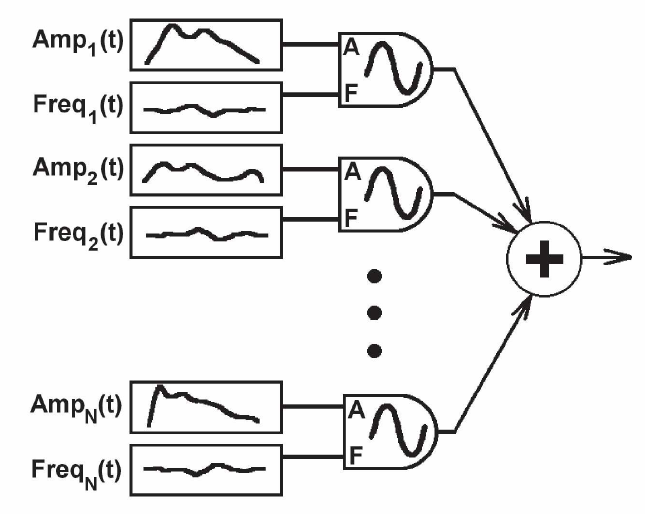
\includegraphics[width=0.5\textwidth]{sinusoidal_add_synth.PNG}
      \caption{Sinusoidal Additive Synthesis Algorithm \cite{Cook:2002:RSS:515316}.}
      \label{fig:sin_add_synth}
\end{figure}

\subsection{Filter-based Modal Synthesis}\label{sec:add_synth}

This method is also additive, since we are adding the outputs of a number of band-pass filters. To synthesize a sound using this method, we use as many filters as the modal frequencies.

\paragraph{Band-pass Filters\\}\label{par:bpf}

At this point we will give some basic description of the band-pass filter since it is widely used in this thesis. Band-pass filters (\gls{BPF}s) take a signal as input and let only a range of frequencies to pass while attenuating the rest. This range depends on the central frequency $f_c$ and the bandwidth. A filter of this kind is a result of a cascading of a low-pass and a high-pass filter circuit.

The \gls{BW} is the passing range or ``band'' of frequencies. Defining as 0db the resonant peak, we can find the two cut-off frequencies ($f_{c,low}$ and $f_{c,high}$) at -3dB. The difference between those two is the bandwidth  
\begin{equation}\label{eq:bw}
BW = f_{c,high}-f_{c,low}.
\end{equation}   
In figure \ref{fig:resp_bpf} we can see the frequency response of a BPF \cite{bib:bpf}. 

\begin{figure}[H]
  \centering
    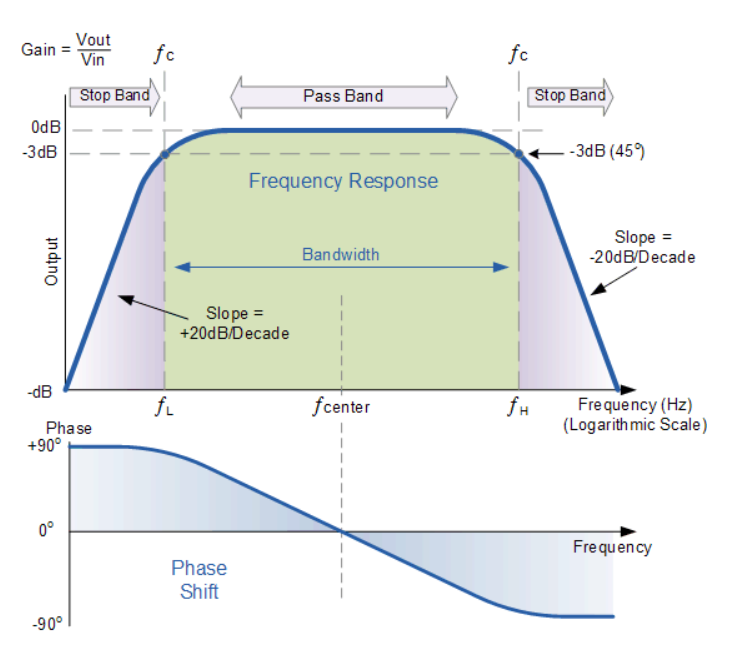
\includegraphics[width=0.7\textwidth]{BPF.PNG}
      \caption{Frequency Response of a Band-pass Filter  \cite{bib:bpf}.}
      \label{fig:resp_bpf}
\end{figure}

\paragraph{Synthesis\\}\label{par:synth}

In this method, a number of filters are constructed using modal frequencies of the object as center frequencies and the damping of the material is used to control the \gls{Q} of the filters.  The \gls{Q} is a dimensionless parameters that is inversely proportional to the bandwidth ($Q=f_c/BW$), so the lower the \gls{Q}, the wider the bandwidth and vice-versa. Using amplitudes from matrix \textbf{A} (section \ref{sec:modal_extraction}), the level of the passing frequencies is controlled and resonators can be created through the sum of these filters. 

\begin{figure}[H]
  \centering
    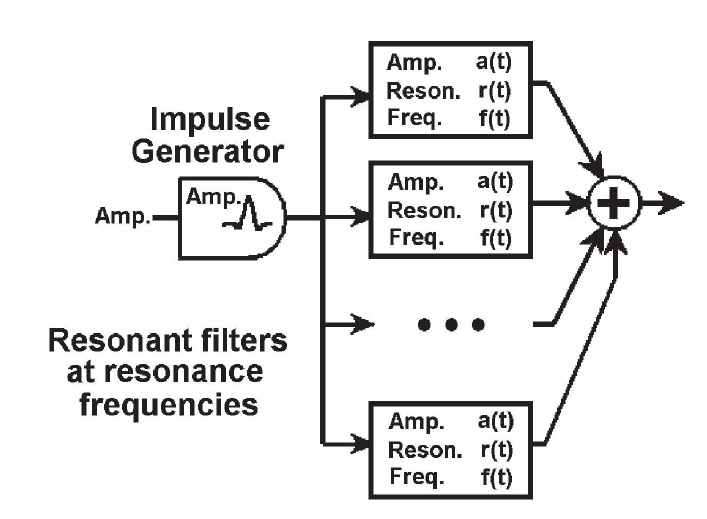
\includegraphics[width=0.5\textwidth]{filter-based_add_synth.PNG}
      \caption{Filter-based Modal Synthesis Algorithm \cite{Cook:2002:RSS:515316}.}
      \label{fig:filter_synth}
\end{figure}

\section{Sound Variations} \label{sec:sound_variation}
Each point of an object produces a different sound when struck. This happens because of the different amount of excitation each resonant mode experiences. As mentioned in section \ref{sec:modal_extraction}, during data extraction we get a matrix of amplitudes of size $K\times N$ corresponding to $K$ different resonant modes of each of the $N$ points of the object. . Note that the frequencies and dampings are determined by the geometry and material properties of the object while the gains of the modes depend on the contact location on the
object \cite{van2001foleyautomatic}. This means that even though resonant frequencies are the same for all surface points, each mode gain is different depending on the location.

There are several methods to achieve spatial variation on sound produced by the same object. 
\begin{itemize}
\item Modal analysis using \gls{FEM} and spring-mass systems (as seen in section \ref{sec:fem} and \ref{sec:springmass})provide the frequencies of resonant filters and the amplitudes for multiple locations on the object (potentially for each vertex). This is why it makes it an accurate method that provides varying sounds along the object's surface. However, as discussed previously, it is not a suitable method for an audio pipeline due to its computational complexity.

\item Another method is to separate the object into areas and assume that each point belonging to the same area and struck with the same force will sound exactly the same. Depending on the resolution of the object's division cells the overall sound of the object varies. The higher the resolution the more varied the sound is and thus the more persuasive results. Additionally, the higher the resolution the more data has to be stored for the model.

\item A third method is to store only one amplitude matrix and randomize the values for each impact sound, but this can lead to  inconsistent sounds with the collision location. For example, impacting the same location with the same force would produce different sounds when theoretically the same sound shoule be heard. This method is used in \cite{lloyd2011sound}.

\item Finally, a better approach to the previous method is to retain the same amplitude values for all points of the object, but apply a texture map on the object which indicates pitch changes of the sound all over the object. For instance, the near-edge points of an object produce a higher-pitched sound than the ones in the center of each faces. 

\end{itemize}

\section{3D Audio}

Spatialized sound is important for 3D virtual worlds because it enables the localization of objects in combination with visual cues. Auditory cues are also essential to localize a sound source that is outside the field of view (i.e. a car driving closer but hidden behind a building corner). Studies show that accurate auditory information increases the sense of presence in a virtual environment \cite{larsson2002better}. Different methods for rendering three-dimensional sound field for the listener's ears are covered in this section.

\subsection{Binaural and transaural techniques}

The aim of these methods is to recreate a wave field at the ears of the listener using most commonly headphones (binaural) or loudspeakers (transaural).

\paragraph{Head-Related Transfer Function\\}\label{par:hrtf}

The goal of \gls{HRTF} is to model, by the use of filters, the effects of resonances inside the ear and close to the head and upper body on sound propagation. To obtain these filters small microphones can be placed at the entrance of a listener's ear canals or on a dummy-head. \gls{HRTF}s vary depending on the individual, due to morphological differences, and depending on the angle of listener's head \cite{zhang2013measurement}, thus they should be adapted for each listener to increase the quality \cite{funkhouser2002sounds}. It is nowadays the most used technique for sound spatialization in combination with head tracking for \gls{VR} and \gls{AR} headsets \cite{bib:hololens, bib:oculus}. 

\paragraph{Transaural stereo\\}\label{par:transaural}

This method makes use of a stereophonic setup of loudspeakers for binaural reproduction. As the signal emitted by the right speaker also reaches the listener's left ear and vice versa, filtering is needed to cancel the cross-talk . Its use is limited to desktop and suffers from a limited sweet-spot, where the binaural reproduction can be acceptable \cite{funkhouser2002sounds}.

\subsection{Multi-channel auditory displays}

These techniques use an array of loudspeakers positioned around the listening area to generate a 3D sound field. They are usually used for larger audiences and suffer from sweet spot problems but on the other hand do not need complex  \gls{HRTF} filtering. VBAP aims at reproducing the auditory cues, utilized by the humans for accurate 3D localization, whereas the Ambisonics and WFS methods aim at reproducing the physical aspects of the sound field. 

\paragraph{Vector-Based Amplitude Panning\\}\label{par:vbap}

\gls{VBAP} is a computationally efficient and accurate method based on auditory perception. By panning the sound sources the perceived source location is shifted. The loudspeakers can be positioned in an arbitrary three-dimentional placement. However it does not allow the reproduction of elevation of the virtual sound source \cite{pulkki1997virtual}.

\paragraph{Ambisonics\\}\label{par:ambisonics}

Ambisonics is a spatial sound encoding method for surround and multi-speaker systems. It uses soundfield microphones that encode audio through an arbitrary number of channels that model the directional soundfield. First order ambisonics make use of four microphones and accuracy increases with the increment of number of microphones used.  Ambisonics has been extended to higher orders to offer more spatial resolution \cite{daniel2003further}. 

\paragraph{Wave Field Synthesis\\}\label{par:wfs}

\gls{WFS} is based on the Kirchoff integral theorem which states that any point of a wave front can be considered as a secondary source. This method requires a large amount (about 120-160 output channels) of loudspeakers, depending on the reproduction area, and processing to give accurate reproduction \cite{funkhouser2002sounds}.

\subsection{3D audio discussion for VR/AR applications}

\gls{WFS} and higher order Ambisonics are multi-user reproduction systems, which could be an interesting element for video games but due to their setup complexity do not seem to be an option for virtual environments. Other methods that make use of loudspeakers offer good spatialization results but are impractical for \gls{VR}/\gls{AR} applications as there should be consistency between the user's viewpoint in the virtual space and the virtual listening location. Additionally, sound reflections on the screen surfaces can engage acoustical problems. This is why binaural systems that use \gls{HRTF} and which are incorporated into nowadays \gls{VR}/\gls{AR} headsets seem to be the best option to maintain consistency between the listener's head motion and the audio scene.